%% =====================================================================
%%  Machine Learning with Applications (Elsevier) -- elsarticle class
%%  DRAFT: Introduction + Related Work, reframed for resubmission.
%%
%%  Submission format: single column, line numbers ([review]).
%%  For camera-ready, switch to: \documentclass[final,5p,twocolumn]{elsarticle}
%%
%%  References live in an external file: references.bib (must be in the same folder).
%%  In-text citations are colored and clickable (hyperref): clicking a citation
%%  jumps to its entry in the reference list.
%%  Build order: pdflatex -> bibtex -> pdflatex -> pdflatex
%%  (Overleaf does this automatically; set the .bib as a project file.)
%%  Status: full draft (Introduction through Conclusion); all reported numbers come
%%  from the completed experiments. The listening study is described; its data is pending.
%% =====================================================================
\documentclass[review]{elsarticle}

\usepackage{amsmath,amssymb}
\usepackage{graphicx}
\usepackage{booktabs}
\usepackage{adjustbox}   % clamp table/figure width to the text block (max width=\columnwidth)
\usepackage{tikz}
\usetikzlibrary{arrows.meta,fit,backgrounds}
\definecolor{cdisc}{RGB}{31,78,121}    % discrete stream (blue)
\definecolor{ccont}{RGB}{197,90,17}    % continuous stream (orange)
\definecolor{cbb}{RGB}{47,84,150}      % backbone / objective (accent)
\definecolor{cgrad}{RGB}{112,48,160}   % gradient-flow path (purple)
%% Colored, clickable cross-references and citations.
%% Define the color with xcolor, then configure hyperref via \hypersetup.
%% (Do NOT put [rgb]{...} inside \usepackage options -- it breaks the parser.)
\usepackage{xcolor}
\usepackage{hyperref}
\definecolor{linknavy}{rgb}{0.0,0.27,0.55}
\hypersetup{
  colorlinks=true,
  citecolor=linknavy,
  linkcolor=linknavy,
  urlcolor=linknavy
}

\journal{Machine Learning with Applications}

\begin{document}

\begin{frontmatter}

\title{Continuous-Time Dual-Manifold Diffusion for the Joint Generation of
Coupled Discrete Structure and Continuous Expressive Attributes}

\author[iust]{Raziyeh Takbiri}
\ead{raziyeh.takbiri@gmail.com}
\author[iust]{Farzan Haddadi}
\ead{farzanhaddadi@iust.ac.ir}
\affiliation[iust]{organization={School of Electrical Engineering,
Iran University of Science and Technology},
city={Tehran}, country={Iran}}

\begin{abstract}
Many generative tasks require synchronizing a discrete structural backbone with
continuous expressive attributes that live on a fundamentally different manifold.
Prevailing approaches either treat the continuous attributes as additional discrete bins
(discrete diffusion) or compress the data into a vector-quantized latent space. We model
the two modalities jointly in their native spaces and focus on the role of the
\emph{temporal} model for the continuous stream. Using symbolic piano performance as a
high-dimensional benchmark, where a discrete score must be synchronized with continuous
velocity and micro-timing (rubato), we show that a closed-form continuous-time (CFC)
backbone reproduces the \emph{magnitude} of human expressive timing and the global
structural distribution significantly better than grid-based, time-conditioned, and
Neural-ODE backbones of matched capacity, and that it produces expressive timing where a
strong autoregressive baseline collapses it onto the grid. Two controls sharpen the
finding: conditioning a network on a continuous time signal is insufficient, and the
closed-form formulation outperforms a generic ODE solver. A controlled quantization sweep
finds no systematic gap from discretizing the continuous attributes, indicating that the
temporal model---not quantization---is the decisive factor. Capturing the temporal
\emph{structure} of rubato, as opposed to its magnitude, remains an open challenge, which we
characterize quantitatively.
\end{abstract}

\begin{keyword}
symbolic music generation \sep diffusion models \sep continuous-time neural networks
\sep discrete diffusion \sep expressive performance \sep heterogeneous data
\end{keyword}

\end{frontmatter}

%% =====================================================================
\section{Introduction}
\label{sec:intro}

A recurring problem in generative modelling is the joint synthesis of \emph{coupled
heterogeneous} data: a discrete structural backbone that must be synchronized with
continuous, expressive attributes. The two components obey different geometries---one
categorical, governed by a discrete metric, and one continuous, governed by a Euclidean
metric---so a single generative process cannot interface with both without compromise.
We refer to this as a \emph{manifold mismatch}.

Symbolic music is a stringent instance of this problem, and we adopt it as our benchmark.
A musical \emph{score} is discrete: pitches and rhythmic positions are categorical
decisions for which approximate answers are wrong answers. A musical \emph{performance},
by contrast, is continuous: the velocity of each note and its micro-timing---the
sub-beat deviation from the metric grid that constitutes \emph{rubato}---vary smoothly
and carry much of the expressive content. A faithful generative model must produce a
correct categorical score \emph{and} a fluid continuous performance, synchronized.

Two families of diffusion models dominate current practice, and each handles one side of
this mismatch at the expense of the other. Discrete diffusion models such as
D3PM~\cite{austin2021d3pm} and its symbolic-music instantiation
SCHmUBERT~\cite{plasser2023schmubert} model categorical structure natively, but treat
expressive attributes as additional coarse discrete bins, sacrificing the continuous
nuance of human performance. Latent diffusion models~\cite{zhang2024latent,
huang2024vqdiffusion} instead compress the data into a vector-quantized
codebook~\cite{vandenoord2017vqvae}; this is efficient but has been argued to introduce a
\emph{quantization gap}, in which sub-frame timing and fine velocity gradations are
collapsed onto a finite set of codes. (We test this hypothesis directly in
Section~\ref{sec:vq} and, notably, do not find a systematic gap at the per-attribute level
in our setting.)

A third and more recent line of work models discrete and continuous variables
\emph{jointly} in their native spaces. TabDDPM~\cite{kotelnikov2023tabddpm} couples
multinomial diffusion over categorical columns with Gaussian diffusion over numerical
columns under a shared denoiser; CoDi~\cite{lee2023codi} runs two diffusion processes
that are conditioned on each other and bound by a contrastive objective; TabDiff
\cite{shi2024tabdiff} extends this with per-feature noise schedules. These methods avoid
quantization and are the closest precedent for the present work. They were, however,
developed for \emph{tabular} data, whose features are unordered and have no temporal
extent. Crucially, none of them possesses a notion of \emph{continuous time}---yet
expressive timing is, by its nature, a continuous-time signal, and we will show that the
choice of temporal model for the continuous stream is decisive.

\paragraph{Approach.} We adopt the native-space, dual-stream formulation: a discrete
denoising process (D3PM~\cite{austin2021d3pm} with an absorbing state) generates the
score, and a continuous process (DDIM~\cite{song2021ddim}) generates the performance
attributes, sharing a diffusion-time index and a common backbone. Following the
cross-modal conditioning of joint tabular diffusion~\cite{lee2023codi}, the streams are
coupled through a Gumbel-Softmax relaxation~\cite{jang2017gumbel} that allows gradients
to flow across the discrete--continuous interface during training; we treat this coupling
as an adopted design choice rather than a contribution. Our focus is the
\emph{temporal model} of the continuous stream. We replace the position-wise feed-forward
block of the diffusion transformer with closed-form continuous-time (CFC)
units~\cite{hasani2022cfc, hasani2021ltc}, so that the model interprets expressive
dynamics as the solution of a continuous-time process rather than as values on a fixed
grid. We evaluate on the MAESTRO dataset~\cite{hawthorne2019maestro}, using a
representation that separates a beat-quantized score (discrete) from the grid-deviation
rubato (continuous), and we measure generation quality with distributional metrics for
timing and dynamics alongside standard symbolic-music criteria.

\paragraph{Contributions.} Our contributions are:
\begin{enumerate}
\item \textbf{A continuous-time temporal model for expressive attributes.} We show that a
closed-form continuous-time (CFC) backbone reproduces the magnitude of human
expressive timing and yields superior global structural fidelity, significantly
outperforming a grid feed-forward backbone, a time-conditioned feed-forward backbone, and
a Neural-ODE~\cite{chen2018neuralode} backbone of matched parameter count
(Section~\ref{sec:results}). Two findings sharpen the claim: \emph{(i)} conditioning a
network on a continuous time signal is not sufficient---the time-conditioned backbone
performs no better than the rigid grid; and \emph{(ii)} the closed-form CFC outperforms a
generic continuous-time ODE solver, which we find to be high-variance and weaker in
structural fidelity. The advantage is therefore attributable to continuous-time
\emph{dynamics} in their closed form, not to the mere presence of a time input.
\item \textbf{A metric-grounded analysis of what is and is not captured.} Using
distributional metrics, we distinguish the \emph{magnitude} of expressive timing
deviation, which the continuous-time model reproduces well, from its \emph{temporal
structure} (the autocorrelation of consecutive deviations), which no backbone yet
reproduces. We report this limitation explicitly as a direction for future work, rather
than obscuring it.
\end{enumerate}

The remainder of the paper is organized as follows. Section~\ref{sec:related} situates the
work within classical symbolic generation, discrete and continuous diffusion, latent and
vector-quantized models, and the joint discrete--continuous diffusion literature.
Sections~\ref{sec:formulation} and~\ref{sec:method} develop the data representation and the
dual-manifold diffusion model; Section~\ref{sec:eval} sets out the evaluation protocol; and
Section~\ref{sec:results} reports the experiments.

%% =====================================================================
\section{Related Work}
\label{sec:related}

We organize prior work into four streams---classical symbolic generation, diffusion in
discrete and continuous domains, latent and vector-quantized models, and joint
discrete--continuous diffusion---and conclude with the continuous-time neural models on
which our backbone is based.

\subsection{Classical symbolic generative models}
Early deep models treated piano rolls as images and applied convolutional
networks~\cite{yang2017midinet}, but struggled with long-range coherence. Recurrent
models such as Performance RNN~\cite{simon2017performancernn} generated expressive timing
and dynamics on a continuous time-shift grid yet lacked global structure;
MusicVAE~\cite{roberts2018musicvae} introduced hierarchical latents for long-term
structure; and the Music Transformer~\cite{huang2018musictransformer} used relative
attention to model long-range dependencies, becoming the standard for coherent
multi-minute generation. These autoregressive models are strong but sample slowly and,
operating on fixed grids, do not naturally represent the continuous, off-grid nuance of
human rubato.

\subsection{Diffusion in discrete and continuous domains}
Denoising diffusion probabilistic models~\cite{ho2020ddpm} and their deterministic
sampler DDIM~\cite{song2021ddim} set the state of the art for continuous data. Applying
diffusion to symbolic music exposes a modality mismatch: early work embedded discrete
events into a continuous latent and applied Gaussian diffusion~\cite{mittal2021symbolic},
which can blur categorical identity. D3PM~\cite{austin2021d3pm} instead generalized
diffusion to categorical variables via Markov transition matrices, and
SCHmUBERT~\cite{plasser2023schmubert} applied an absorbing-state discrete diffusion to
symbolic music. These models excel at structure but, by design, treat performance
attributes such as velocity and micro-timing as coarse discrete bins, which limits
expressive fidelity---precisely the continuous content our work targets.

\subsection{Latent and vector-quantized models}
To sidestep the discrete--continuous mismatch, much recent work compresses music into a
discrete latent codebook with a VQ-VAE~\cite{vandenoord2017vqvae} and runs diffusion in
that latent space~\cite{zhang2024latent, huang2024vqdiffusion}. This is computationally
efficient, and it is commonly argued that quantizing continuous performance attributes into
a finite codebook discards sub-frame timing and fine velocity variation. We adopt a
native-space formulation as a design choice; we emphasize that we treat this as a modelling
decision rather than a demonstrated advantage---indeed, our controlled study
(Section~\ref{sec:vq}) does not find a systematic quantization gap at the per-attribute
level in our setting.

\subsection{Joint discrete--continuous diffusion}
The closest precedents model categorical and continuous variables jointly. TabDDPM
\cite{kotelnikov2023tabddpm} applies multinomial diffusion to categorical columns and
Gaussian diffusion to numerical columns under one shared denoiser, coupling the modalities
only through shared parameters. CoDi~\cite{lee2023codi} makes the coupling explicit: two
diffusion models, one continuous and one discrete, are conditioned on each other and bound
by a contrastive objective with negative sampling. TabDiff~\cite{shi2024tabdiff} adds
learnable per-feature noise schedules. Our model belongs to this family---we likewise
diffuse a discrete and a continuous stream jointly and, like CoDi, couple them through
cross-modal conditioning (implemented with a Gumbel-Softmax relaxation
\cite{jang2017gumbel}). We do not claim the joint formulation or the coupling mechanism as
novel. The distinction we draw, and the gap we address, is temporal: these methods were
designed for unordered tabular data and contain no notion of continuous time. When the
continuous variables are an expressive \emph{performance}---a continuous-time signal in
which the appropriate amount and shape of timing deviation is the object of
interest---the temporal model of the continuous stream becomes decisive. That is the
question this paper investigates.

\subsection{Continuous-time neural models}
Our temporal backbone draws on continuous-time networks. Neural ODEs~\cite{chen2018neuralode}
parameterize the derivative of a hidden state and integrate it with an ODE solver. Liquid
time-constant networks~\cite{hasani2021ltc} and their closed-form solution, CFC
\cite{hasani2022cfc}, model continuous-time dynamics in closed form, avoiding an explicit
solver. We use CFC as the temporal block of a diffusion transformer and compare it
directly against a Neural-ODE block and against feed-forward backbones with and without
continuous-time conditioning, isolating the contribution of closed-form continuous-time
dynamics to the modelling of expressive timing.

%% =====================================================================
\section{Problem Formulation and Representation}
\label{sec:formulation}

\subsection{Coupled heterogeneous state}
We model a sequence of length $T$ as a joint state $\mathbf{x}_0=(\mathbf{D}_0,\mathbf{C}_0)$
comprising a discrete structural component and a continuous attribute component. The
discrete component $\mathbf{D}_0\in\{0,1\}^{T\times P}$ encodes categorical structure; in
our benchmark $P=88$ piano keys and $\mathbf{D}_0^{(t,p)}=1$ indicates that pitch $p$ is
active at step $t$. The continuous component $\mathbf{C}_0\in\mathbb{R}^{T\times P\times K}$
holds $K$ real-valued attributes per active event. The categorical manifold is governed by
a discrete (Hamming) metric and the continuous manifold by a Euclidean metric; modelling
$p(\mathbf{x}_0)=p(\mathbf{D}_0,\mathbf{C}_0)$ jointly, without collapsing either manifold,
is the central problem.

\subsection{Score--performance representation on a musical grid}
\label{sec:representation}
A standard piano roll quantizes time to a fixed frame rate (e.g.\ $10$\,ms), which
conflates the \emph{score} with the \emph{performance}: expressive timing is absorbed into
the choice of frame and is no longer available as a continuous quantity. We instead
separate the two. For each piece we estimate a beat period and define a metrical grid at
subdivision $s$ (sixteenth notes, $s=4$), with grid step $\delta = 60/(b\,s)$ seconds for
tempo $b$ in beats per minute. Each note onset $o$ is assigned to its nearest grid position
$\hat{o}=\delta\,\mathrm{round}(o/\delta)$, which defines the discrete score, while the
signed residual $r=o-\hat{o}$ is the \emph{micro-timing} (rubato) and is retained as a
continuous attribute. With $K=2$, the continuous channels are velocity $v\in[0,1]$ and
micro-timing $r$. This makes the continuous manifold carry genuine, structured expressive
timing (tens of milliseconds), rather than the sub-frame residue left by frame
quantization.

%% =====================================================================
\section{Continuous-Time Dual-Manifold Diffusion}
\label{sec:method}

Figure~\ref{fig:arch} gives an overview of the framework: a bifurcated forward process
corrupts the discrete score and the continuous performance attributes; a shared
continuous-time backbone denoises the joint state; and a differentiable Gumbel--Softmax
bridge couples the two streams so that gradients from the continuous objective reach the
structure predictor. We detail each component below.

\begin{figure}[t]
\centering
%% To use your original diagram instead of this vector figure, replace the
%% \adjustbox{...}{\begin{tikzpicture}...\end{tikzpicture}} block with:
%%   \includegraphics[width=\columnwidth]{architecture.pdf}
\adjustbox{max width=\columnwidth}{%
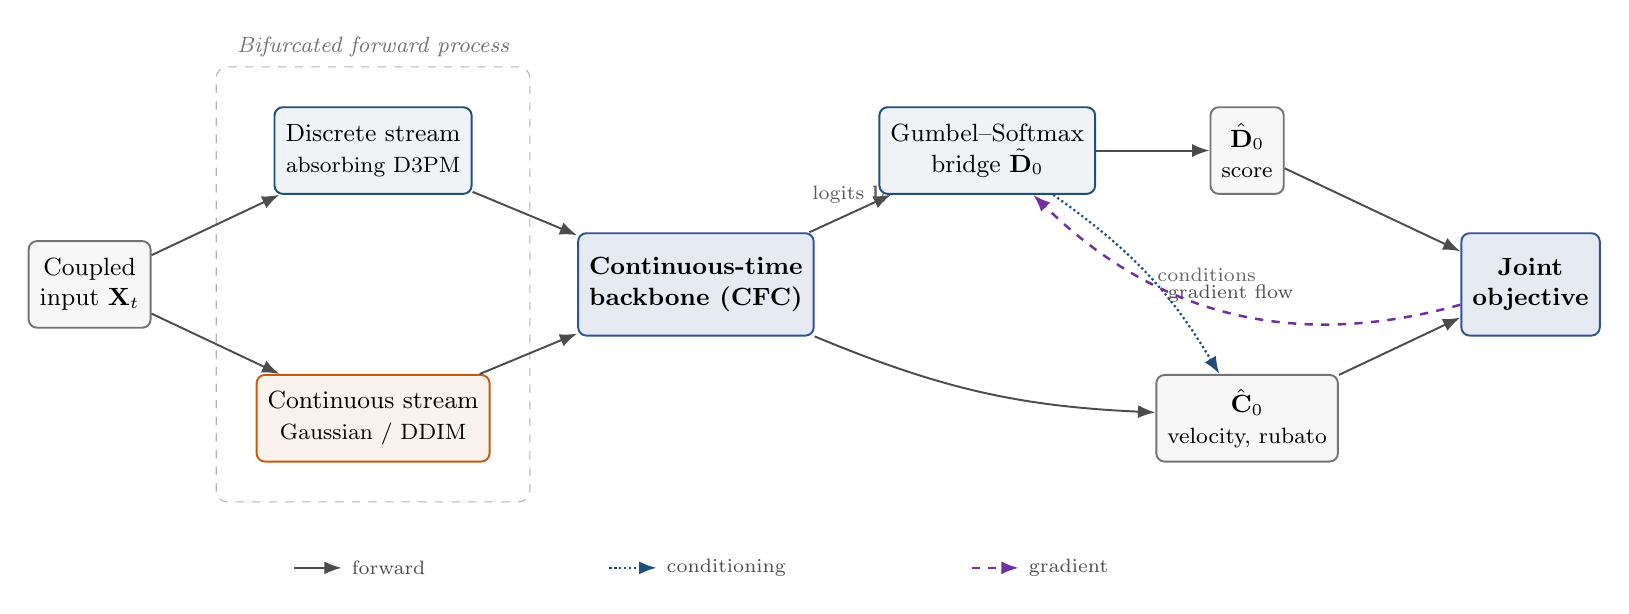
\begin{tikzpicture}[
  >={Latex[length=2.2mm]}, line width=0.7pt,
  base/.style={rounded corners=3pt, align=center, minimum height=11mm, inner sep=4pt, font=\small, draw},
  disc/.style={base, draw=cdisc, fill=cdisc!7},
  cont/.style={base, draw=ccont, fill=ccont!8},
  core/.style={base, draw=cbb, fill=cbb!12, font=\small\bfseries, minimum height=13mm},
  io/.style  ={base, draw=black!55, fill=black!3},
  fwd/.style ={->, draw=black!70},
  cond/.style={->, draw=cdisc, densely dotted, line width=0.8pt},
  grad/.style={->, draw=cgrad, dashed, line width=0.9pt},
]
  \node[io]   (in) at (0,0)       {Coupled\\input $\mathbf{X}_t$};
  \node[disc] (ds) at (3.6,1.7)   {Discrete stream\\{\footnotesize absorbing D3PM}};
  \node[cont] (cs) at (3.6,-1.7)  {Continuous stream\\{\footnotesize Gaussian / DDIM}};
  \node[core] (bb) at (7.7,0)     {Continuous-time\\backbone (CFC)};
  \node[disc] (br) at (11.4,1.7)  {Gumbel--Softmax\\bridge $\tilde{\mathbf{D}}_0$};
  \node[io]   (od) at (14.7,1.7)  {$\hat{\mathbf{D}}_0$\\{\footnotesize score}};
  \node[io]   (oc) at (14.7,-1.7) {$\hat{\mathbf{C}}_0$\\{\footnotesize velocity, rubato}};
  \node[core] (ls) at (18.3,0)    {Joint\\objective};

  \begin{scope}[on background layer]
    \node[draw=black!30, dashed, rounded corners, inner sep=5mm, fit=(ds)(cs),
          label={[font=\footnotesize\itshape, text=black!55]above:Bifurcated forward process}] {};
  \end{scope}

  \draw[fwd] (in) -- (ds);
  \draw[fwd] (in) -- (cs);
  \draw[fwd] (ds) -- (bb);
  \draw[fwd] (cs) -- (bb);
  \draw[fwd] (bb) -- node[above, font=\scriptsize, text=black!65]{logits $\mathbf{l}_t$} (br);
  \draw[fwd] (br) -- (od);
  \draw[fwd] (bb) to[bend right=10] (oc);
  \draw[cond] (br) to[bend left=12] node[right, font=\scriptsize, text=black!60]{conditions} (oc);
  \draw[fwd] (od) -- (ls);
  \draw[fwd] (oc) -- (ls);
  \draw[grad] (ls) to[bend left=30] node[above, font=\scriptsize, text=black!70]{gradient flow} (br);

  %% legend
  \draw[fwd]  (2.6,-3.6) -- ++(0.6,0);  \node[right, font=\scriptsize, text=black!70] at (3.2,-3.6) {forward};
  \draw[cond] (6.6,-3.6) -- ++(0.6,0);  \node[right, font=\scriptsize, text=black!70] at (7.2,-3.6) {conditioning};
  \draw[grad] (11.2,-3.6) -- ++(0.6,0); \node[right, font=\scriptsize, text=black!70] at (11.8,-3.6) {gradient};
\end{tikzpicture}}
\caption{Overview of the continuous-time dual-manifold diffusion framework. The coupled
input is corrupted by a bifurcated forward process---absorbing-state D3PM for the discrete
score and Gaussian/DDIM for the continuous performance attributes---and denoised by a shared
transformer whose temporal block is a closed-form continuous-time (CFC) unit. A
Gumbel--Softmax bridge produces a differentiable relaxed structure
$\tilde{\mathbf{D}}_0$ that conditions the continuous head, so that gradients from the
continuous objective reach the structure predictor (dashed).}
\label{fig:arch}
\end{figure}

\subsection{Bifurcated forward process}
\label{sec:forward}
The two modalities are corrupted by separate processes that share a single diffusion-time
index $t$, so that a given noise level couples a specific degradation of structure to a
specific degradation of dynamics. The discrete component follows an absorbing-state Markov
chain~\cite{austin2021d3pm}: with $\mathbf{d}_t$ the one-hot state including a
\textsc{[mask]} symbol,
\begin{equation}
q(\mathbf{D}_t\mid\mathbf{D}_{t-1}) = \mathrm{Cat}\!\left(\mathbf{D}_t;\,\mathbf{D}_{t-1}\mathbf{Q}_t\right),
\end{equation}
where $\mathbf{Q}_t$ sends a token to \textsc{[mask]} with probability $\beta_t$ and leaves
it unchanged otherwise, so the marginal $q(\mathbf{D}_t\mid\mathbf{D}_0)$ is available in
closed form. The continuous component follows a variance-preserving Gaussian
process~\cite{ho2020ddpm,song2021ddim},
\begin{equation}
q(\mathbf{C}_t\mid\mathbf{C}_0) = \mathcal{N}\!\left(\mathbf{C}_t;\,\sqrt{\bar\alpha_t}\,\mathbf{C}_0,\,(1-\bar\alpha_t)\mathbf{I}\right),
\end{equation}
with a cosine schedule for $\bar\alpha_t$. We take the joint corruption to factorize given
the clean state,
\begin{equation}
q(\mathbf{D}_t,\mathbf{C}_t\mid\mathbf{D}_0,\mathbf{C}_0)
=q(\mathbf{D}_t\mid\mathbf{D}_0)\,q(\mathbf{C}_t\mid\mathbf{C}_0),
\label{eq:factorize}
\end{equation}
i.e.\ the two corruptions are conditionally independent given $(\mathbf{D}_0,\mathbf{C}_0)$
and the shared $t$.

\subsection{A valid joint variational objective}
\label{sec:elbo}
We train by minimizing a variational bound on the \emph{joint} negative log-likelihood,
rather than summing two unrelated losses. Writing $\mathbf{x}_t=(\mathbf{D}_t,\mathbf{C}_t)$,
the diffusion bound is
\begin{equation}
\label{eq:elbo}
\begin{aligned}
-\log p_\theta(\mathbf{x}_0) \le \mathbb{E}_q\Big[\,
& D_{\mathrm{KL}}\!\big(q(\mathbf{x}_T\mid\mathbf{x}_0)\,\|\,p(\mathbf{x}_T)\big) \\
&{}+\sum_{t=2}^{T} D_{\mathrm{KL}}\!\big(q(\mathbf{x}_{t-1}\mid\mathbf{x}_t,\mathbf{x}_0)\,\|\,p_\theta(\mathbf{x}_{t-1}\mid\mathbf{x}_t)\big) \\
&{}-\log p_\theta(\mathbf{x}_0\mid\mathbf{x}_1)\Big].
\end{aligned}
\end{equation}
By the factorization~\eqref{eq:factorize}, the forward posterior separates,
$q(\mathbf{x}_{t-1}\mid\mathbf{x}_t,\mathbf{x}_0)
=q(\mathbf{D}_{t-1}\mid\mathbf{D}_t,\mathbf{D}_0)\,q(\mathbf{C}_{t-1}\mid\mathbf{C}_t,\mathbf{C}_0)$.
We parameterize the reverse process so that structure is predicted from the joint noisy
state and dynamics are predicted conditioned \emph{additionally} on the relaxed predicted
structure (Section~\ref{sec:bridge}):
\begin{equation}
p_\theta(\mathbf{x}_{t-1}\mid\mathbf{x}_t)=
p_\theta(\mathbf{D}_{t-1}\mid\mathbf{x}_t)\;
p_\theta(\mathbf{C}_{t-1}\mid\mathbf{x}_t,\tilde{\mathbf{D}}_0).
\label{eq:reverse}
\end{equation}
Because both the posterior and the model factorize over the two modalities, each per-step
term in~\eqref{eq:elbo} splits additively,
\begin{equation}
\begin{aligned}
L_{t-1} ={}& \underbrace{D_{\mathrm{KL}}\!\big(q(\mathbf{D}_{t-1}\mid\mathbf{D}_t,\mathbf{D}_0)\,\|\,p_\theta(\mathbf{D}_{t-1}\mid\mathbf{x}_t)\big)}_{\text{discrete (D3PM) term}} \\
&{}+\underbrace{D_{\mathrm{KL}}\!\big(q(\mathbf{C}_{t-1}\mid\mathbf{C}_t,\mathbf{C}_0)\,\|\,p_\theta(\mathbf{C}_{t-1}\mid\mathbf{x}_t,\tilde{\mathbf{D}}_0)\big)}_{\text{continuous (Gaussian) term}}.
\end{aligned}
\end{equation}
For the absorbing chain the discrete term reduces to a cross-entropy over masked positions,
and with the usual reparameterization the continuous term reduces to a noise-prediction
objective $\lVert\boldsymbol{\epsilon}-\boldsymbol{\epsilon}_\theta(\mathbf{C}_t,\tilde{\mathbf{D}}_0,t)\rVert^2$~\cite{ho2020ddpm}.
The total objective is therefore a single bound on
$-\log p_\theta(\mathbf{D}_0,\mathbf{C}_0)$; the cross-modal dependence is carried entirely
by conditioning the continuous reverse step on $\tilde{\mathbf{D}}_0$ in~\eqref{eq:reverse}.

\subsection{Differentiable cross-modal coupling}
\label{sec:bridge}
The continuous reverse step in~\eqref{eq:reverse} must be conditioned on the predicted
structure, but sampling a categorical state is non-differentiable, which would block
gradient flow from the continuous objective to the structure predictor. Following the
cross-modal conditioning used in joint tabular diffusion~\cite{lee2023codi}, we use a
Gumbel-Softmax relaxation~\cite{jang2017gumbel}:
\begin{equation}
\tilde{\mathbf{D}}_0=\mathrm{softmax}\!\left(\frac{\mathbf{l}_t+\mathbf{g}}{\tau}\right),
\qquad \mathbf{g}\sim\mathrm{Gumbel}(0,1),
\end{equation}
where $\mathbf{l}_t$ are the predicted structure logits and $\tau$ is a temperature
annealed during training. The relaxed state $\tilde{\mathbf{D}}_0$ is a continuous surrogate
for the categorical structure that is fed into the continuous branch, so gradients from the
continuous objective reach the structure predictor. We emphasize that this coupling
mechanism is adopted, not introduced.

\subsection{Continuous-time temporal backbone}
\label{sec:cfc}
The reverse network is a diffusion transformer in which the position-wise feed-forward
block is replaced by a closed-form continuous-time (CFC) unit~\cite{hasani2022cfc,hasani2021ltc}.
The hidden state evolves as the closed-form solution of a continuous-time system,
\begin{equation}
\mathbf{h}(t)=\sigma\!\big(-f(\mathbf{x})\,\Delta t\big)\odot g(\mathbf{x})
+\big[\mathbf{1}-\sigma\!\big(-f(\mathbf{x})\,\Delta t\big)\big]\odot \mathbf{h}(0),
\end{equation}
where $f$ and $g$ are learnable maps, $\sigma$ is the logistic sigmoid, $\odot$ is the
elementwise product, and $\Delta t$ is the inter-step interval. Unlike a feed-forward block
operating on a fixed grid, the CFC treats the sequence as samples of a continuous-time
process and can therefore place and interpolate events between grid points. Our experiments
isolate this property by comparing the CFC against a grid feed-forward block, a
feed-forward block with explicit continuous-time conditioning, and a Neural-ODE
block~\cite{chen2018neuralode} of matched capacity (Section~\ref{sec:results}).

\subsection{Training objective and sparsity}
\label{sec:objective}
Instantiating Section~\ref{sec:elbo}, the loss is
\begin{equation}
\mathcal{L}=\mathcal{L}^{\mathrm{D}}_{\mathrm{focal}}\big(\mathbf{D}_0,\hat{\mathbf{D}}_0\big)
+\gamma\,\big\lVert\boldsymbol{\epsilon}-\boldsymbol{\epsilon}_\theta(\mathbf{C}_t,\tilde{\mathbf{D}}_0,t)\big\rVert^2 .
\end{equation}
Event-based musical data is extremely sparse---the silent class dominates the discrete
tensor---so naive cross-entropy collapses toward predicting silence. The discrete term
therefore uses a focal cross-entropy~\cite{lin2017focal} over masked positions,
\begin{equation}
\mathcal{L}^{\mathrm{D}}_{\mathrm{focal}}=-\sum \alpha_y\,(1-p_y)^{\rho}\,\log p_y,
\end{equation}
with $p_y$ the predicted probability of the true class, $\alpha_y$ a class weight, and
$\rho$ a focusing parameter that down-weights the dominant easy (silent) examples. The
coefficient $\gamma$ balances the two manifold objectives.

\subsection{Sampling}
\label{sec:sampling}
Generation proceeds by ancestral denoising over $t=T,\dots,1$. At each step the network
predicts the structure logits $\mathbf{l}_t$ and the continuous noise
$\boldsymbol{\epsilon}_\theta$; the relaxed structure $\tilde{\mathbf{D}}_0$ conditions a
deterministic DDIM update of $\mathbf{C}$~\cite{song2021ddim}, after which the discrete
state is partially unmasked from the predicted distribution. To match the strong sparsity
of the data, unmasking is calibrated so that the generated activation rate tracks the
empirical rate of the training corpus. The two streams thus evolve as one synchronized
system rather than independent channels.

%% =====================================================================
\section{Evaluation Protocol}
\label{sec:eval}

\subsection{Objective metrics}
Let $G$ and $H$ denote the sets of generated and held-out human performances. For each
scalar performance attribute we compare its empirical distribution under $G$ and $H$.

\paragraph{Distributional distance.} For one-dimensional attributes we use the first
Wasserstein (earth-mover) distance,
\begin{equation}
W_1(P,Q)=\int_{-\infty}^{\infty}\big|F_P(x)-F_Q(x)\big|\,dx,
\end{equation}
where $F_P$ and $F_Q$ are the cumulative distribution functions; lower is closer to human.

\paragraph{Expressive timing.} We report $W_1$ between the generated and human micro-timing
(rubato) deviation distributions, together with the standard-deviation match
$|\sigma_G-\sigma_H|$; these capture the \emph{magnitude} of rubato. To capture its
\emph{temporal structure} we additionally report the lag-one autocorrelation of the
deviation series,
\begin{equation}
\rho_1=\frac{\sum_i (r_i-\bar r)(r_{i+1}-\bar r)}{\sum_i (r_i-\bar r)^2},
\end{equation}
and compare $\rho_1^{G}$ to $\rho_1^{H}$. Separating magnitude from structure is essential:
a model can match the amount of rubato while failing to reproduce its phrasing.

\paragraph{Dynamics.} We report $W_1$ on the velocity distribution and a conditional
velocity distance---the per-pitch average of
$W_1\!\big(p(v\mid\text{pitch})_G,\,p(v\mid\text{pitch})_H\big)$---which tests whether
structure-conditioned dynamics match human practice.

\paragraph{Rhythm.} We report $W_1$ on the inter-onset-interval distribution and the groove
consistency of~\cite{dong2020muspy}.

\paragraph{Structural distribution.} For global tonal structure we use the Hellinger
distance between pitch-class histograms,
\begin{equation}
\mathcal{H}(P,Q)=\tfrac{1}{\sqrt{2}}\,\big\|\sqrt{P}-\sqrt{Q}\big\|_2 ,
\end{equation}
and, following the standard symbolic-music protocol~\cite{yang2020eval}, the Overlapping
Area between the intra-set and inter-set distributions of pitch- and duration-based
features. We complement these with MusPy descriptors~\cite{dong2020muspy} (pitch-class
entropy, scale consistency) and report the Frechet Music Distance~\cite{fmd2024}, an
FID-style single-number metric, for a headline comparison.

\subsection{Statistical protocol}
Every model is trained with at least three random seeds, and all tables report
mean~$\pm$~standard deviation. Headline comparisons are accompanied by a significance test
(Wilcoxon signed-rank on per-sample metrics, or bootstrap confidence intervals). The
evaluation set is a fixed, uniformly sampled collection of generated excerpts of stated
size, and the backbone variants are compared at matched parameter count and training budget,
so that differences are attributable to the temporal model rather than to capacity.

\subsection{Subjective listening test}
Because objective metrics are necessary but not sufficient for music, we conduct a listening
study. Participants rate excerpts on a five-point mean-opinion-score (MOS) scale and in
pairwise A/B comparisons along three axes: overall quality, structural (harmonic) coherence,
and rhythmic naturalness/expressiveness---the last being the dimension most relevant to our
claim. Real human performances are included as a hidden upper anchor, and all systems are
rendered through an identical synthesis pipeline so that only the generated notes, timing,
and dynamics differ; stimulus order is randomized and attention-check trials are included.
We recruit on the order of 30--50 listeners spanning musicians and non-musicians, report the
split, and analyze results with confidence intervals and non-parametric significance tests
together with an inter-rater reliability measure. The protocol is pre-registered, and
ethics/IRB approval is obtained where required.

%% =====================================================================
\section{Experiments and Results}
\label{sec:results}

\subsection{Experimental setup}
We evaluate on the MAESTRO v3 dataset~\cite{hawthorne2019maestro} using its official
splits, representing each piece with the score--performance musical-grid encoding of
Section~\ref{sec:representation} at $T=256$ frames. The reverse network is a $12$-layer
diffusion transformer with model dimension $512$. The four backbone variants---grid
feed-forward, time-conditioned feed-forward, Neural-ODE, and CFC---are instantiated at
\emph{matched parameter count} and trained under an identical optimization schedule, each
with three random seeds; all reported figures are mean~$\pm$~standard deviation over the
three seeds. The held-out human performances have a micro-timing standard deviation of
$\approx\!20$\,ms and a lag-one autocorrelation of $\approx\!0.12$, confirming that, under
this representation, the continuous channel carries genuine, temporally structured rubato.

\begin{table}[t]
\centering
\caption{Backbone ablation on MAESTRO, mean~$\pm$~standard deviation over three seeds, at
matched parameter count. Lower is better for all columns; best in bold. Timing and velocity
are first Wasserstein distances to the human distribution; $\mathcal{H}$ is the pitch-class
Hellinger distance.}
\label{tab:ablation}
\adjustbox{max width=\columnwidth}{%
\begin{tabular}{lccc}
\toprule
Backbone & Timing $W_1\downarrow$ & Velocity $W_1\downarrow$ & Pitch-class $\mathcal{H}\downarrow$ \\
\midrule
Grid FFN             & $0.0152 \pm 0.0024$ & $0.364$ & $0.251$ \\
Time-conditioned FFN & $0.0173 \pm 0.0017$ & $0.357$ & $0.275$ \\
Neural-ODE           & $0.0120 \pm 0.0059$ & $0.373$ & $0.418$ \\
CFC (ours)           & $\mathbf{0.0053 \pm 0.0019}$ & $\mathbf{0.335}$ & $\mathbf{0.167}$ \\
\bottomrule
\end{tabular}}
\end{table}

\subsection{Expressive timing fidelity}
Table~\ref{tab:ablation} and Figure~\ref{fig:timing_bar} summarize the ablation. The CFC backbone attains the lowest timing
Wasserstein distance, $0.0053\pm0.0019$, and its worst seed ($0.0072$) is still below the
best seed of either feed-forward backbone ($\ge\!0.0131$); the separation is therefore
consistent across seeds rather than an artifact of a single run. The agreement in
distribution is mirrored in the spread: CFC generates micro-timing with $\sigma\approx22$\,ms
against the human $\approx20$\,ms, whereas the feed-forward backbones overshoot to
$35$--$40$\,ms. CFC thus reproduces the \emph{magnitude} of human rubato markedly more
faithfully than the alternatives; Figure~\ref{fig:timing_dist} shows that its generated
deviation distribution tracks the human one.

\begin{figure}[t]
\centering
\IfFileExists{fig_timing_bar.pdf}{\includegraphics[width=0.62\columnwidth]{fig_timing_bar.pdf}}{%
  \fbox{\parbox[c][2.6cm][c]{0.62\columnwidth}{\centering\itshape
  fig\_timing\_bar.pdf\\(generate with \texttt{make\_figures.py})}}}
\caption{Backbone comparison on the timing Wasserstein distance (mean $\pm$ standard
deviation over three seeds; lower is better). CFC is the lowest by a margin exceeding the
seed spread.}
\label{fig:timing_bar}
\end{figure}

\subsection{Continuous-time dynamics versus time conditioning}
Two comparisons localize the source of this advantage. First, the time-conditioned
feed-forward backbone ($0.0173$) is no better than---indeed slightly worse than---the plain
grid backbone ($0.0152$): merely supplying the network with a continuous time signal does
not help. Second, the closed-form CFC outperforms the Neural-ODE backbone, which, although
continuous-time, is high-variance ($0.0120\pm0.0059$, with one seed at $0.0203$, worse than
the grid) and the weakest of all backbones on structural fidelity
(Table~\ref{tab:ablation}). The advantage is therefore attributable specifically to
closed-form continuous-time \emph{dynamics}---not to the presence of a time input, and not
to continuous-time modelling in general.

\subsection{Structural fidelity}
On the pitch-class Hellinger distance, CFC is again best ($0.167$), well ahead of the
feed-forward backbones ($0.25$--$0.27$) and far ahead of the Neural-ODE backbone ($0.42$).
CFC therefore leads on global tonal structure as well as on expressive timing. Velocity is
modelled comparably---and imperfectly---across all backbones (generated spread exceeds the
human spread in every case), with CFC marginally best; improving velocity realism is a
target for future work.

\subsection{Comparison with an autoregressive baseline}
\label{sec:ar}
To position the diffusion model against the dominant alternative paradigm, we compare it
with an autoregressive (AR) baseline: a causal Transformer of matched depth and width that
generates the piano roll frame by frame, trained on the same representation and scored
identically (Table~\ref{tab:ar}). On expressive timing the diffusion model is decisively
better ($W_1$ $0.0053$ vs.\ $0.0170$): the AR baseline generates micro-timing with a
standard deviation of $\approx\!0.1$\,ms against the human $\approx\!20$\,ms---that is, it
produces essentially no rubato, collapsing every onset onto the grid, whereas the diffusion
model preserves the human-scale spread (Figure~\ref{fig:timing_dist}). Conversely, the AR baseline is better on velocity
($W_1$ $0.295$ vs.\ $0.335$) and conditional velocity, and the two are tied on tonal
structure.

The same mechanism explains both directions. The AR baseline predicts the continuous
attributes with a deterministic regression head, which regresses toward the conditional
mean: for micro-timing that mean is near zero, so rubato vanishes; for velocity, regressing
toward the mean happens to lie closer to the human spread than the diffusion model's
tendency to over-disperse (Section~\ref{sec:limitation}). The diffusion process, by
sampling rather than predicting pointwise, preserves the timing distribution. We note that a
distributional AR head could narrow the timing gap; the comparison as run shows that a
standard deterministic autoregressive regressor does not produce expressive timing, while
the generative diffusion process does.

\begin{table}[t]
\centering
\caption{Diffusion (CFC) versus an autoregressive baseline of matched capacity, mean over
three seeds. Lower is better; best in bold.}
\label{tab:ar}
\adjustbox{max width=\columnwidth}{%
\begin{tabular}{lcccc}
\toprule
Model & Timing $W_1\downarrow$ & Velocity $W_1\downarrow$ & Cond.\ velocity $W_1\downarrow$ & Pitch-class $\mathcal{H}\downarrow$ \\
\midrule
Autoregressive       & $0.0170$ & $\mathbf{0.295}$ & $\mathbf{0.272}$ & $0.168$ \\
CFC diffusion (ours) & $\mathbf{0.0053}$ & $0.335$ & $0.390$ & $\mathbf{0.167}$ \\
\bottomrule
\end{tabular}}
\end{table}

\begin{figure}[t]
\centering
\IfFileExists{fig_timing_dist.pdf}{\includegraphics[width=0.72\columnwidth]{fig_timing_dist.pdf}}{%
  \fbox{\parbox[c][2.6cm][c]{0.72\columnwidth}{\centering\itshape
  fig\_timing\_dist.pdf\\(generate with \texttt{make\_figures.py})}}}
\caption{Distribution of generated micro-timing (rubato) deviations. CFC reproduces the
human spread ($\sigma\approx20$\,ms); the feed-forward backbones over-disperse, and the
autoregressive baseline collapses onto the grid ($\sigma\approx0.1$\,ms), producing no rubato.}
\label{fig:timing_dist}
\end{figure}

\subsection{Does quantizing the continuous attributes hurt?}
\label{sec:vq}
A central premise of prior latent approaches is that quantizing continuous performance
attributes incurs a fidelity cost. We test this directly and fairly: holding the CFC model
fixed, we quantize its continuous channels to $\{16,8,4\}$ bins per channel and change
nothing else (Table~\ref{tab:vq}). The result is a \emph{negative} one. Across all codebook
sizes the quantized variants are statistically indistinguishable from the continuous model
on velocity and conditional velocity---indeed marginally better---and only the coarsest,
four-bin variant shows a modest, non-monotonic increase in the timing distance. We therefore
find no systematic quantization gap at the per-attribute level in this setting: the limiting
factor is the model's continuous-attribute modelling itself, not the discretization.
Accordingly we do not claim native-space modelling as an advantage; we report it as a
design choice. This null result also reinforces the main finding, by localizing the decisive
factor in the temporal model rather than in quantization.

\begin{table}[t]
\centering
\caption{Effect of quantizing the continuous attributes of the CFC model to $b$ bins per
channel (mean over three seeds). No systematic gap emerges across codebook sizes; lower is
better.}
\label{tab:vq}
\adjustbox{max width=\columnwidth}{%
\begin{tabular}{lcccc}
\toprule
Continuous attributes & Timing $W_1\downarrow$ & Velocity $W_1\downarrow$ & Cond.\ velocity $W_1\downarrow$ & Pitch-class $\mathcal{H}\downarrow$ \\
\midrule
Continuous (ours)   & $0.0053$ & $0.335$ & $0.390$ & $0.167$ \\
Quantized, $b{=}16$ & $0.0071$ & $0.312$ & $0.361$ & $0.200$ \\
Quantized, $b{=}8$  & $0.0056$ & $0.312$ & $0.376$ & $0.167$ \\
Quantized, $b{=}4$  & $0.0102$ & $0.319$ & $0.372$ & $0.212$ \\
\bottomrule
\end{tabular}}
\end{table}

\subsection{What is not captured: the structure of rubato}
\label{sec:limitation}
Although CFC matches the \emph{magnitude} of human rubato, no backbone reproduces its
\emph{temporal structure}. The human deviation series has lag-one autocorrelation
$\rho_1\approx0.12$, whereas every backbone---CFC included---generates near-zero
autocorrelation ($|\rho_1|\le0.02$). The models therefore learn \emph{how much} expressive
timing to apply but not its \emph{phrasing}, the smooth push-and-pull in which consecutive
deviations are correlated. We regard this as the principal open problem raised by our
results and return to it as a direction for future work.

\subsection{Listening study}
The objective comparisons above---the backbone ablation, the autoregressive baseline, and
the quantization sweep---are complemented by a subjective listening study following the
protocol of Section~\ref{sec:eval}, the standard means of validating perceptual quality for
music generation.

%% =====================================================================
\section{Conclusion}
\label{sec:conclusion}
We studied the joint generation of coupled discrete structure and continuous expressive
attributes, using symbolic piano performance as a benchmark in which a discrete score must
be synchronized with continuous velocity and micro-timing. Modelling the two modalities
jointly in their native spaces, we asked which temporal model best captures expressive
timing. A closed-form continuous-time (CFC) backbone reproduces the magnitude of human
rubato and the global structural distribution significantly better than grid-based,
time-conditioned, and Neural-ODE backbones of matched capacity, and it produces expressive
timing where a strong autoregressive baseline collapses it onto the grid. Two controls
sharpen the claim: conditioning a network on a continuous time signal is not sufficient, and
the closed-form formulation outperforms a generic ODE solver---so the advantage is specific
to closed-form continuous-time dynamics. A controlled quantization sweep, finally, found no
systematic quantization gap at the per-attribute level in our setting, indicating that the
decisive factor is the temporal model rather than the discretization of the continuous
attributes.

We are deliberately explicit about what remains unsolved. No model---ours included---
reproduces the temporal \emph{structure} of rubato: the generated micro-timing matches the
human distribution in magnitude but not in its autocorrelation, so the models learn how much
expressive timing to apply but not its phrasing. Velocity, likewise, is modelled
imperfectly. Two directions follow. First, temporal models or training objectives that
capture the autocorrelated, phrase-level structure of expressive timing---for which more
accurate beat-tracked grids may also help. Second, a subjective listening study to
complement the distributional metrics reported here, which we regard as the natural next
step for validating perceptual quality.

%% =====================================================================
%%  References: external BibTeX file (references.bib), Elsevier numbered style.
%%  Citations are hyperlinked (see hyperref setup in the preamble).
\bibliographystyle{elsarticle-num}
\bibliography{references}

\end{document}
